
\section{Análisis comparativo entre TCP y gRPC}
\label{sec:comparacion-tcp-grpc}

Una vez implementados los mecanismos de comunicación mediante sockets TCP y
gRPC, se realizó un análisis comparativo para observar cómo se comportan
ambos cuando intercambian mensajes entre los tres nodos del sistema. Para
ello, se utilizaron los resultados obtenidos durante los experimentos,
considerando principalmente la latencia, el throughput y las solicitudes
concurrentes.

El propósito de esta comparación es identificar las diferencias observadas
entre las dos implementaciones bajo las condiciones de prueba utilizadas,
sin asumir que los resultados necesariamente serán iguales en otros equipos
o entornos de red.

\subsection{Metodología del análisis comparativo}

Ambos mecanismos se midieron en el mismo equipo, sobre \texttt{localhost},
con tres nodos, los mismos tamaños de carga útil (100 y 10.240 bytes), cinco
repeticiones de cien muestras por tamaño y una prueba de tres solicitudes
concurrentes. Estas condiciones permiten comparar las corridas registradas,
aunque no eliminan toda variación temporal del equipo.

Para realizar la comparación se utilizaron los archivos
\texttt{data/tcp\_latency.csv} y \texttt{data/grpc\_latency.csv}, que
contienen las mediciones obtenidas con cada mecanismo.

Se trabajó con dos tamaños de mensaje: uno corto de 100 bytes y otro largo
de 10.240 bytes. Para cada combinación se realizaron cinco repeticiones
de cien muestras, por lo que se obtuvieron 500 mediciones para TCP y
otras 500 para gRPC en cada tamaño.

En total, se analizaron 2.000 registros de latencia. A partir de estos
datos se calcularon la media, mediana, mínimo, máximo, desviación estándar,
percentil 95 (P95) y throughput promedio.

También se calcularon intervalos de confianza estimados del 95\,\% para
las medias y para las diferencias observadas entre los mecanismos. Estos
valores permiten apreciar la variabilidad de las mediciones, aunque su
interpretación debe considerar que las muestras proceden de repeticiones
de una misma configuración experimental.

El procesamiento se realizó mediante el módulo
\texttt{analysis/compare\_tcp\_grpc.py}, que genera los archivos CSV y
los gráficos utilizados en esta sección.

\subsection{Comparación de latencia}

La latencia representa el tiempo que tarda una comunicación en completar
el intercambio de solicitud y respuesta. Esta métrica permite observar
cuánto tiempo necesita cada mecanismo para realizar una comunicación
bajo las condiciones de las pruebas.

En la Tabla~\ref{tab:comparacion-latencia} se presentan los resultados
obtenidos para los dos tamaños de mensaje.

\begin{table}[htbp]
\centering
\caption{Comparación estadística de latencia entre TCP y gRPC}
\label{tab:comparacion-latencia}
\begin{tabular}{llrrr}
\hline
\textbf{Tamaño} & \textbf{Mecanismo} &
\textbf{Muestras} & \textbf{Media (ms)} &
\textbf{P95 (ms)} \\
\hline
Corto & TCP  & 500 & 7,220525 & 13,501700 \\
Corto & gRPC & 500 & 3,634639 & 5,048150 \\
Largo & TCP  & 500 & 4,850986 & 7,165695 \\
Largo & gRPC & 500 & 3,271925 & 5,009995 \\
\hline
\end{tabular}
\end{table}

Los resultados muestran que gRPC registró una latencia media menor en
ambos tamaños de mensaje. Para los mensajes cortos, la diferencia fue
de aproximadamente 3,59 ms, mientras que para los mensajes largos fue
de 1,58 ms.

En términos porcentuales, la reducción observada de latencia con gRPC
fue del 49,66\,\% para los mensajes cortos y del 32,55\,\% para los
largos, tomando como referencia los valores medios de TCP.

Un detalle que también llama la atención es que, en esta ejecución,
los mensajes largos presentaron una latencia media menor que los cortos
en ambos mecanismos. Esto demuestra que el tamaño del mensaje no fue
el único factor que intervino en los tiempos registrados.


\begin{table}[htbp]
\centering
\caption{Intervalos de confianza estimados de las diferencias de latencia}
\label{tab:intervalos-confianza}
\begin{tabular}{lrr}
\hline
\textbf{Tamaño} & \textbf{Límite inferior (ms)} &
\textbf{Límite superior (ms)} \\
\hline
Corto & 3,226532 & 3,945241 \\
Largo & 1,244700 & 1,913422 \\
\hline
\end{tabular}
\end{table}

Los intervalos estimados muestran que, en las dos categorías,
la diferencia media observada favoreció a gRPC. Estos valores
deben interpretarse considerando los supuestos estadísticos
del cálculo y la posible dependencia entre las mediciones
de una misma corrida.


\subsection{Comparación del throughput}

Además de la latencia, se comparó el throughput promedio, que representa
la cantidad de mensajes procesados por segundo según las mediciones
registradas durante los experimentos.

\begin{table}[htbp]
\centering
\caption{Throughput promedio por mecanismo y tamaño de mensaje}
\label{tab:comparacion-throughput}
\begin{tabular}{lrrr}
\hline
\textbf{Tamaño} & \textbf{TCP (msg/s)} &
\textbf{gRPC (msg/s)} & \textbf{Variación (\%)} \\
\hline
Corto & 144,301253 & 275,372357 & 90,83 \\
Largo & 204,265171 & 306,316840 & 49,96 \\
\hline
\end{tabular}
\end{table}

En los dos tamaños de mensaje, gRPC obtuvo un throughput promedio
superior al registrado con TCP. La diferencia fue más amplia para
los mensajes cortos, donde el valor de gRPC fue aproximadamente un
90,83\,\% mayor.

Para los mensajes largos también se observó una diferencia favorable
a gRPC, con un incremento del 49,96\,\%.

Estos resultados muestran que, durante las corridas realizadas,
gRPC procesó una mayor cantidad de mensajes por segundo según la
métrica utilizada. Sin embargo, este comportamiento corresponde
a la configuración experimental evaluada y no debe considerarse
una ventaja garantizada en cualquier escenario.

\subsection{Comportamiento ante solicitudes concurrentes}

También se compararon los resultados de las pruebas de concurrencia.
En esta parte se realizaron tres comunicaciones simultáneas entre
los nodos A, B y C, registrando el tiempo de respuesta de cada una.

\begin{table}[htbp]
\centering
\caption{Resultados de las pruebas de concurrencia}
\label{tab:comparacion-concurrencia}
\begin{tabular}{lrrr}
\hline
\textbf{Métrica} & \textbf{TCP} & \textbf{gRPC} &
\textbf{Unidad} \\
\hline
Solicitudes & 3 & 3 & -- \\
Respuestas exitosas & 3 & 3 & -- \\
Latencia media & 6,335300 & 13,068033 & ms \\
Latencia mínima & 6,115400 & 12,071400 & ms \\
Latencia máxima & 6,678700 & 13,938400 & ms \\
Desviación estándar & 0,301274 & 0,939883 & ms \\
\hline
\end{tabular}
\end{table}

A diferencia de los resultados de latencia individual, en esta prueba
TCP presentó un tiempo medio de respuesta menor que gRPC. Los tres
mecanismos de comunicación completaron correctamente sus solicitudes,
por lo que ambas implementaciones respondieron ante las comunicaciones
simultáneas realizadas.

Este resultado es importante porque permite observar que el
comportamiento de los mecanismos puede cambiar según el tipo de prueba.
Aunque gRPC obtuvo mejores valores en las mediciones de latencia y
throughput, TCP registró menor tiempo de respuesta en esta prueba
concurrente.

De todas formas, se debe considerar que solamente se utilizaron tres
solicitudes. Por esta razón, no sería correcto afirmar que TCP tiene
mejor escalabilidad a partir de estos resultados.

\subsection{Visualización de los resultados}

El gráfico de barras de latencia incluye intervalos de confianza estimados
del 95\,\% para las medias de cada grupo.

\begin{figure}[htbp]
\centering
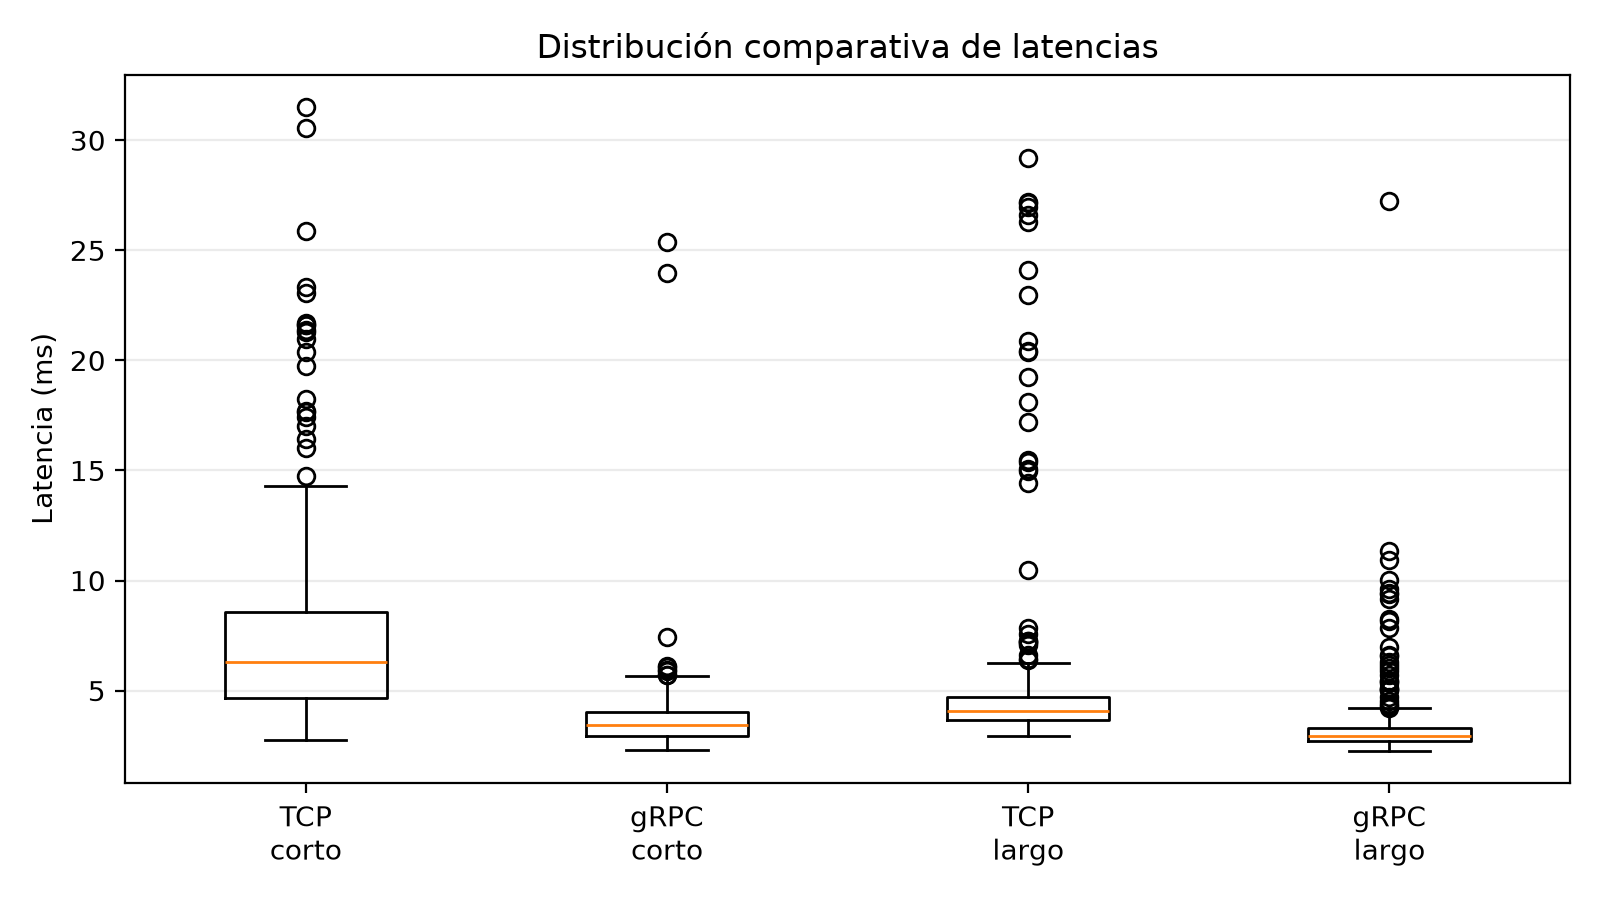
\includegraphics[width=0.85\linewidth]{analysis/figures/comparative_boxplot.png}
\caption{Diagramas de caja de las latencias TCP y gRPC por tamaño de mensaje.}
\label{fig:comparative-boxplot}
\end{figure}

Para facilitar la interpretación de los datos, el programa de análisis
generó tres gráficos que permiten observar las diferencias entre TCP
y gRPC.

\begin{figure}[htbp]
\centering
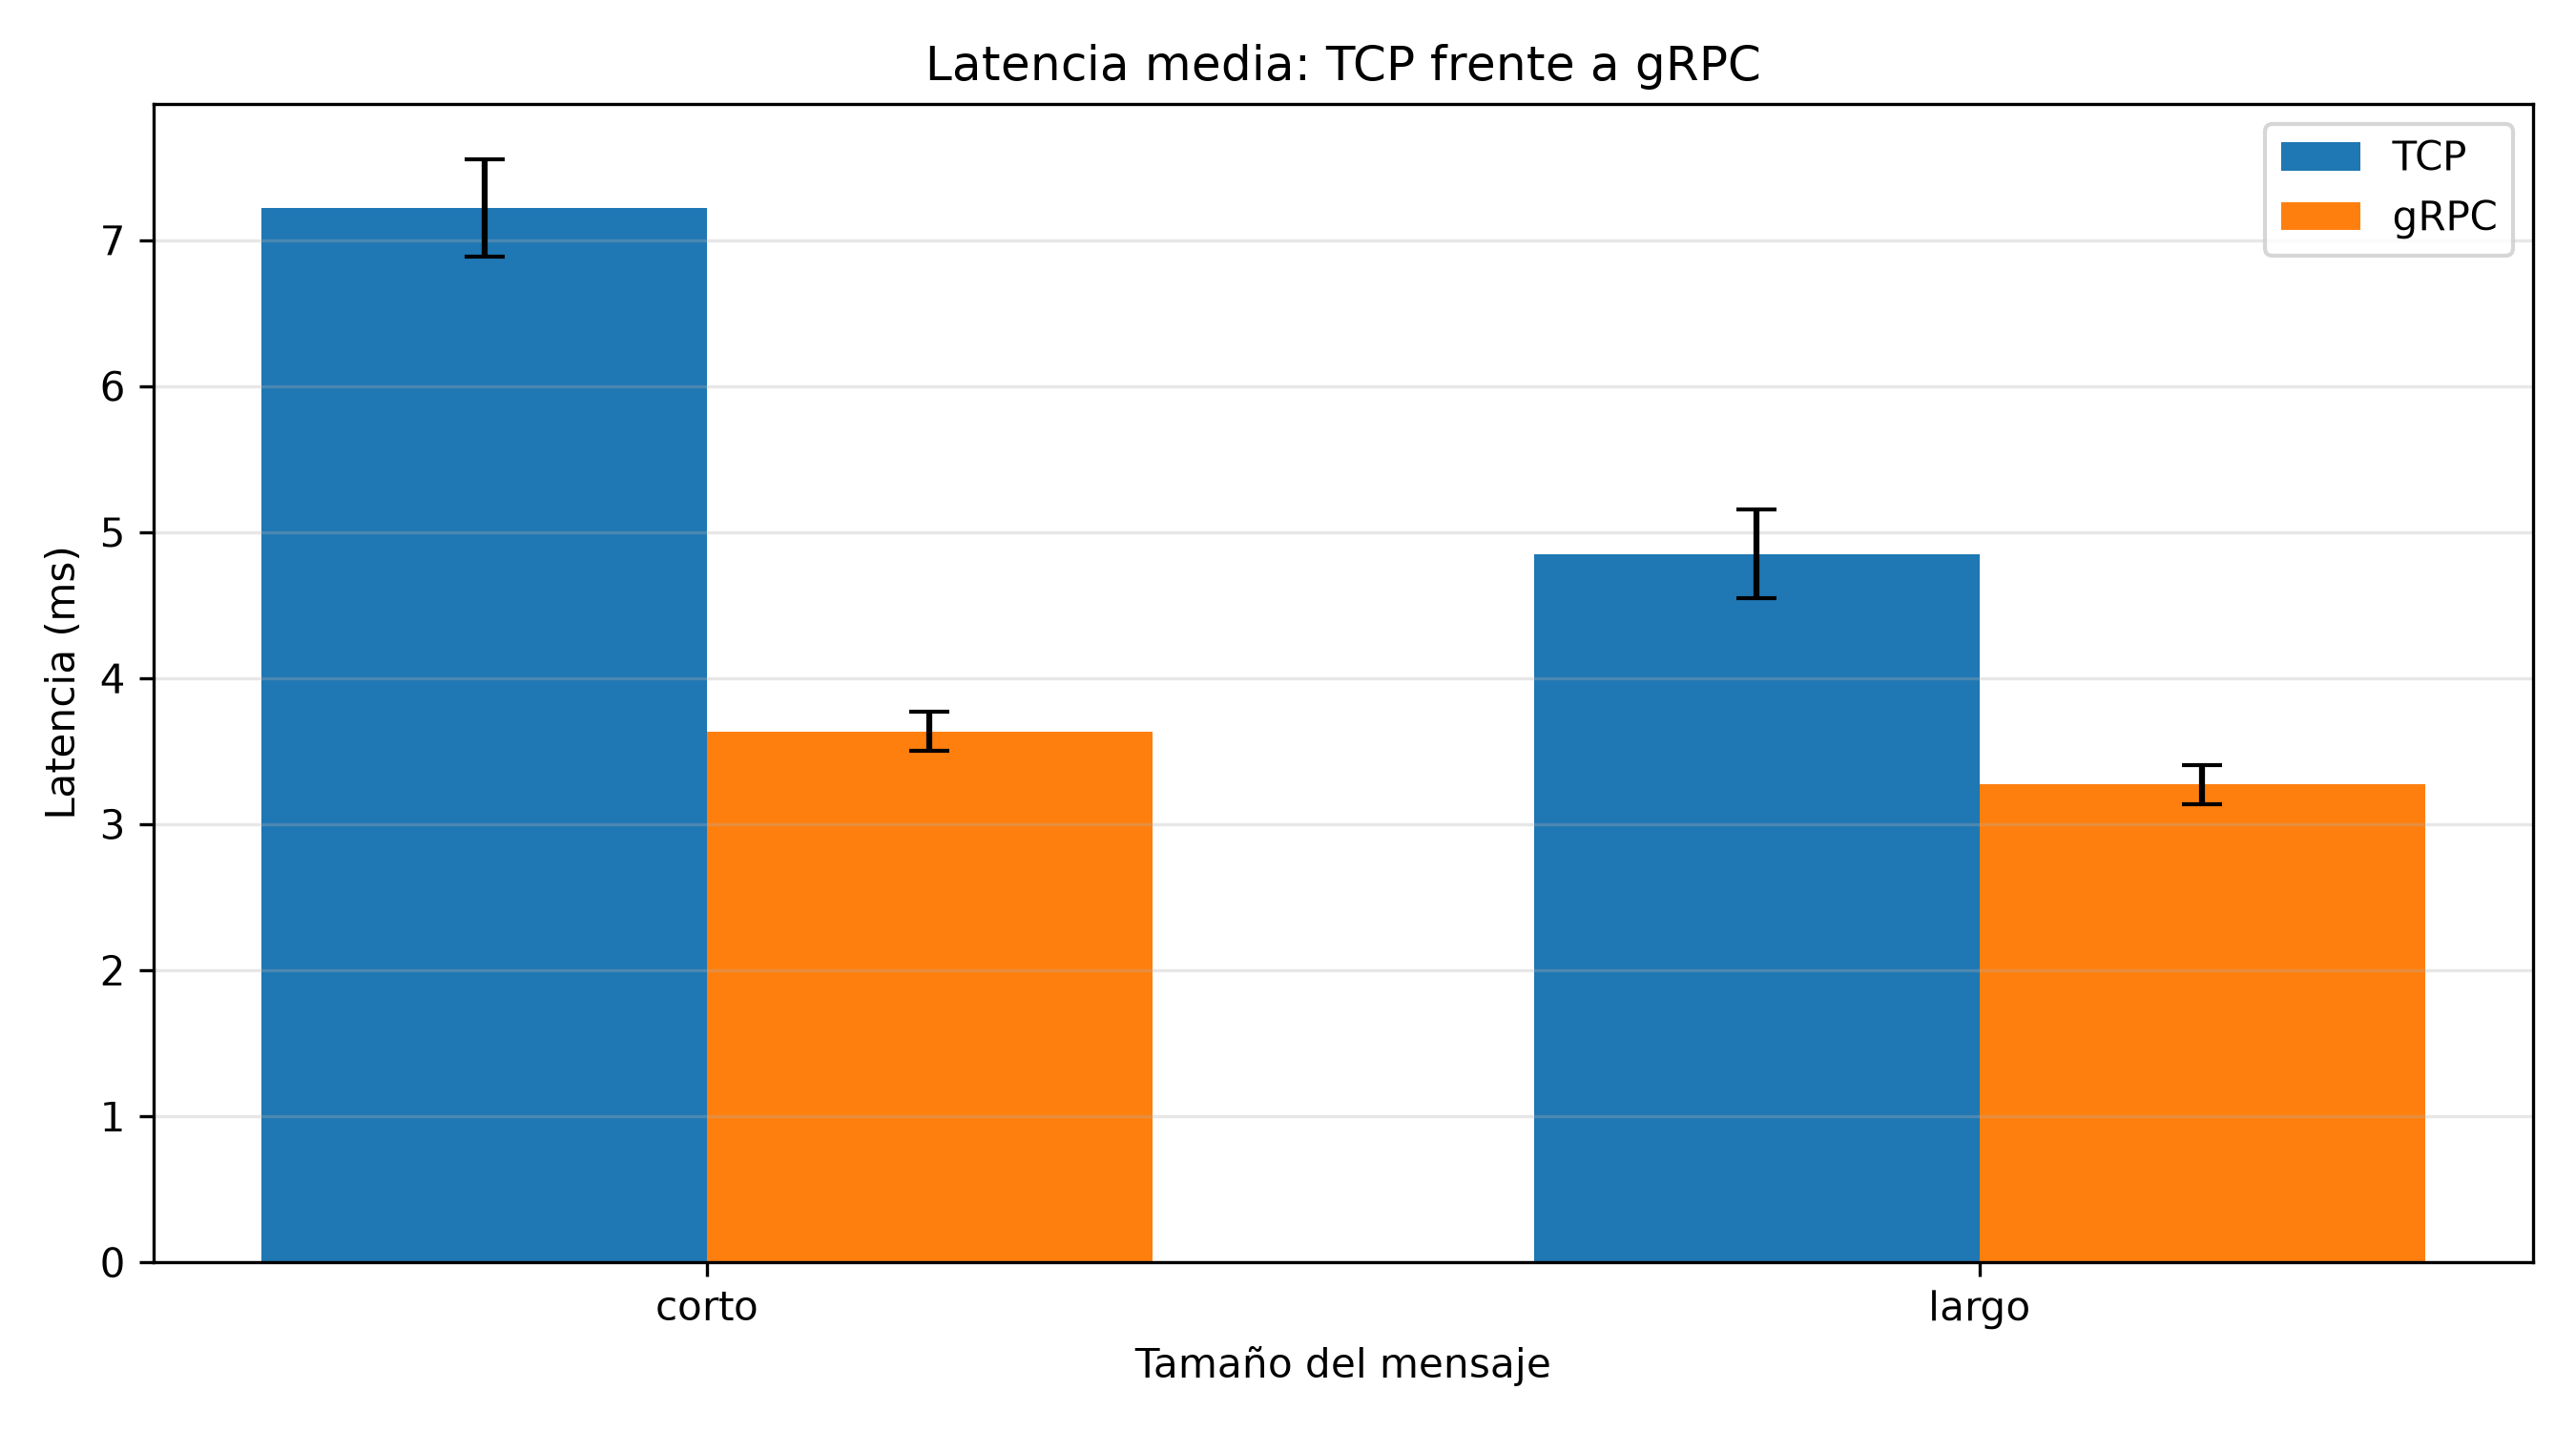
\includegraphics[width=0.85\linewidth]
{analysis/figures/comparative_latency.png}
\caption{Comparación de latencia entre TCP y gRPC.}
\label{fig:comparative-latency}
\end{figure}

La Figura~\ref{fig:comparative-latency} permite observar las diferencias
entre las latencias medias de ambos mecanismos para los dos tamaños
de mensaje. En esta ejecución, gRPC presentó valores inferiores en
ambos casos.

\begin{figure}[htbp]
\centering
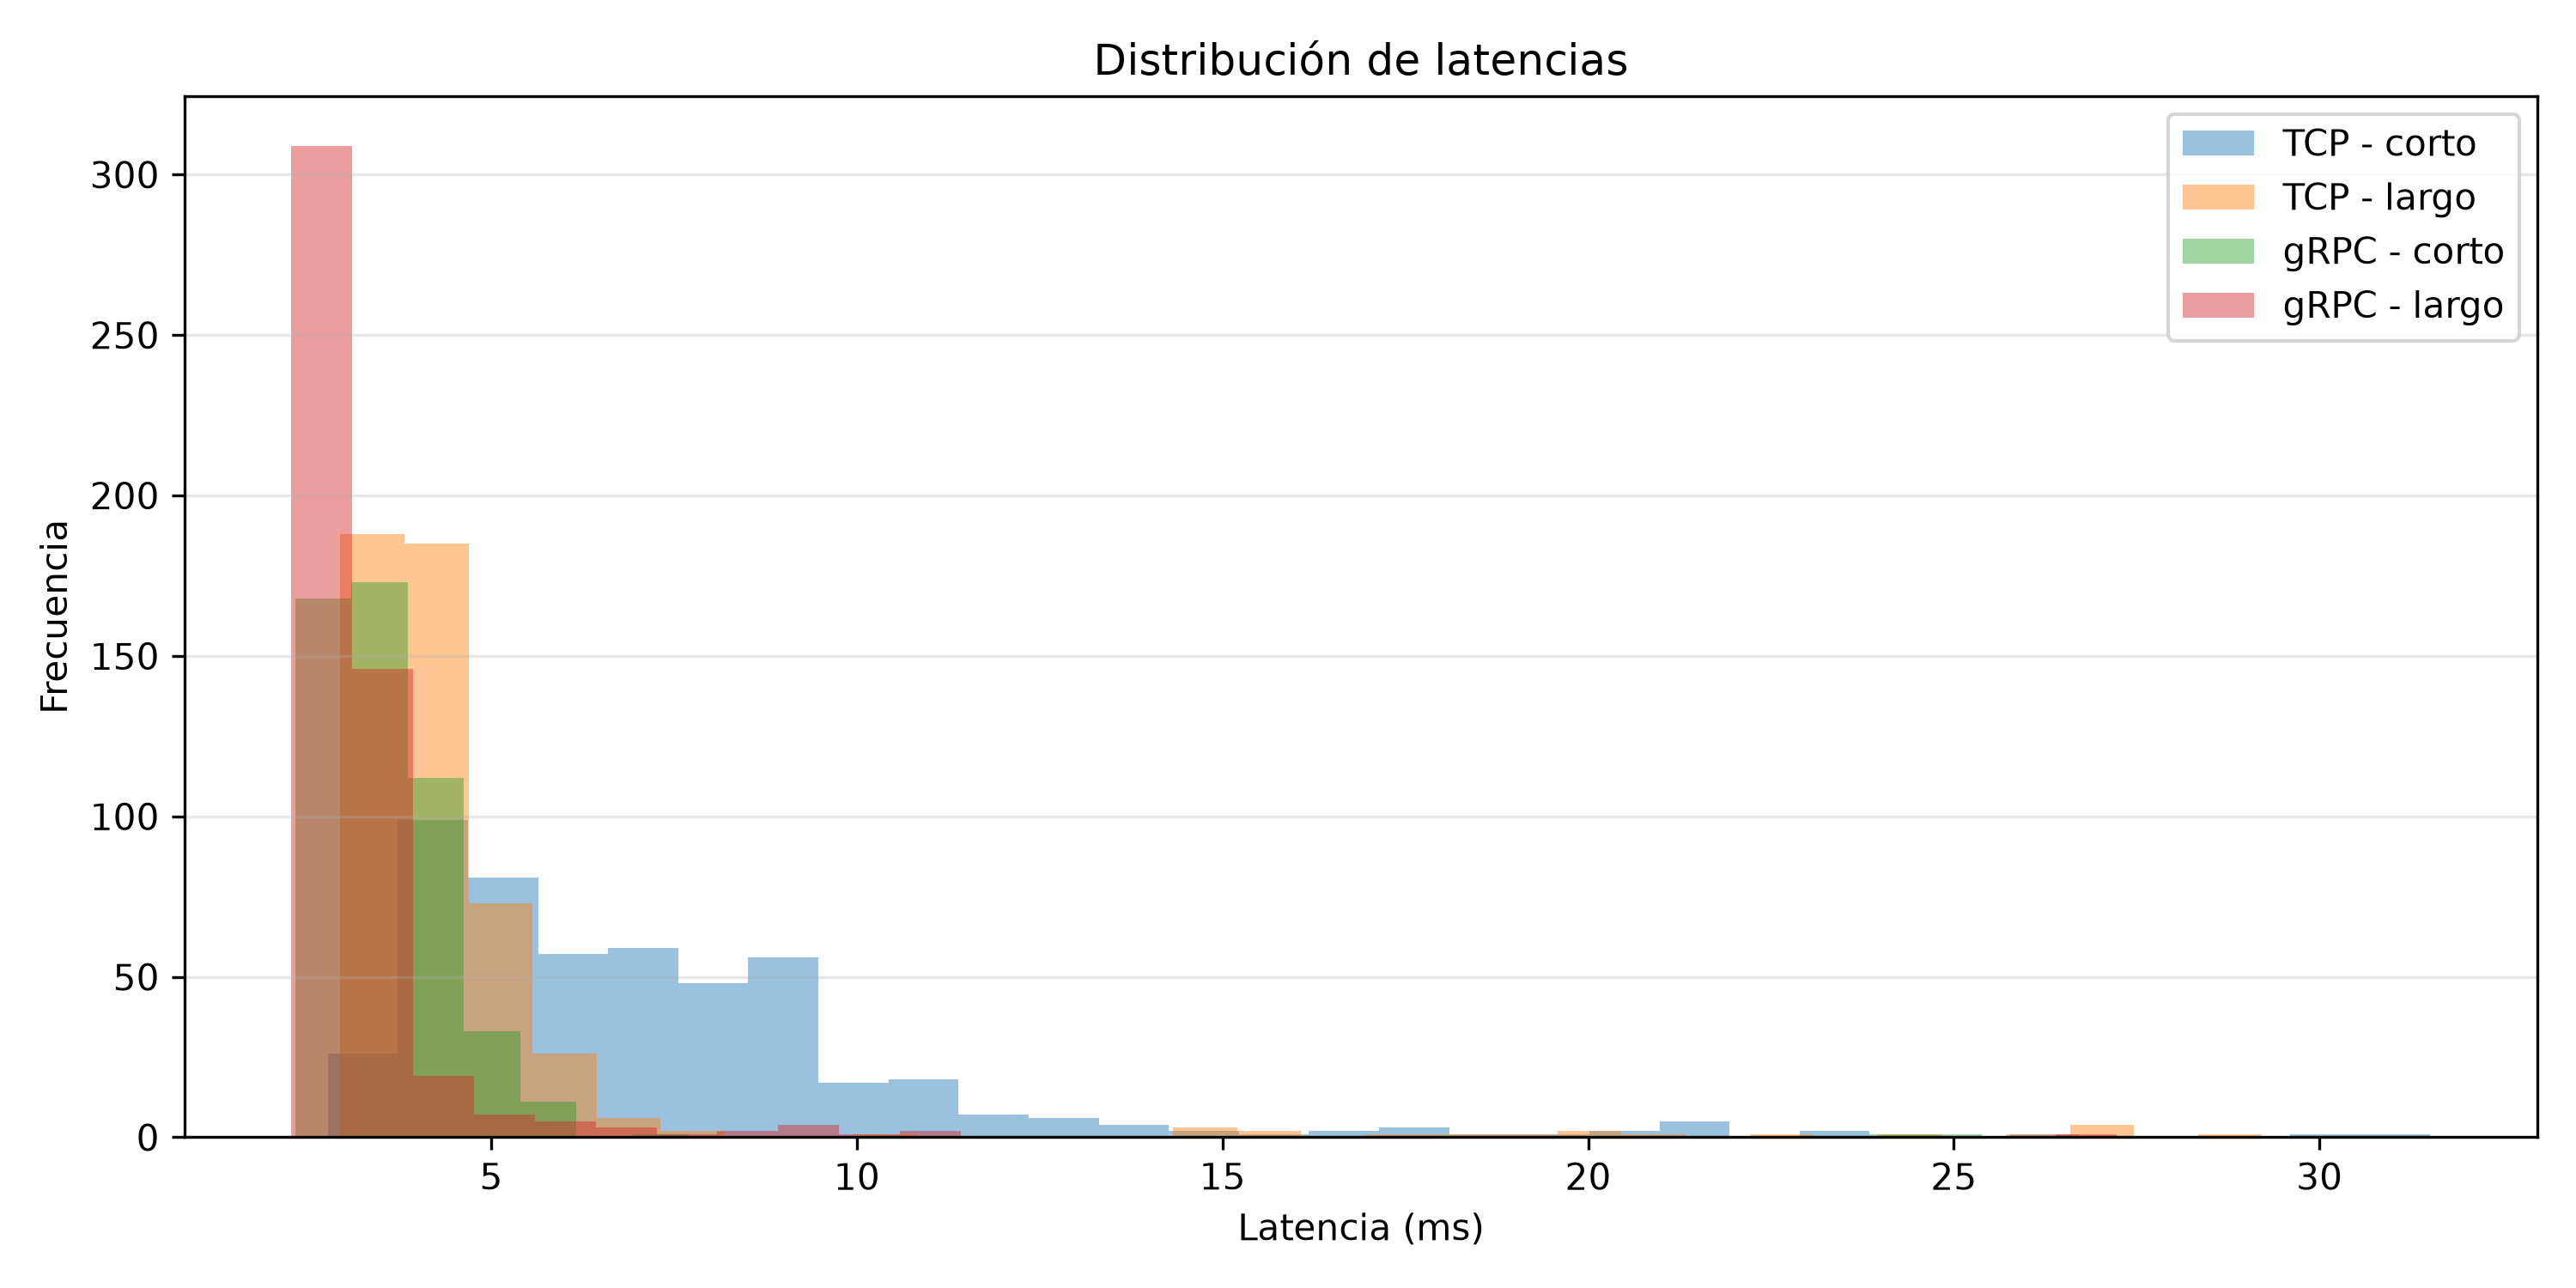
\includegraphics[width=0.85\linewidth]
{analysis/figures/comparative_distribution.png}
\caption{Distribución de las latencias registradas.}
\label{fig:comparative-distribution}
\end{figure}

En la Figura~\ref{fig:comparative-distribution} se puede observar cómo
se distribuyeron las mediciones de latencia. Esta representación
complementa los valores medios, ya que permite apreciar la dispersión
de los tiempos registrados durante los experimentos.

\begin{figure}[htbp]
\centering
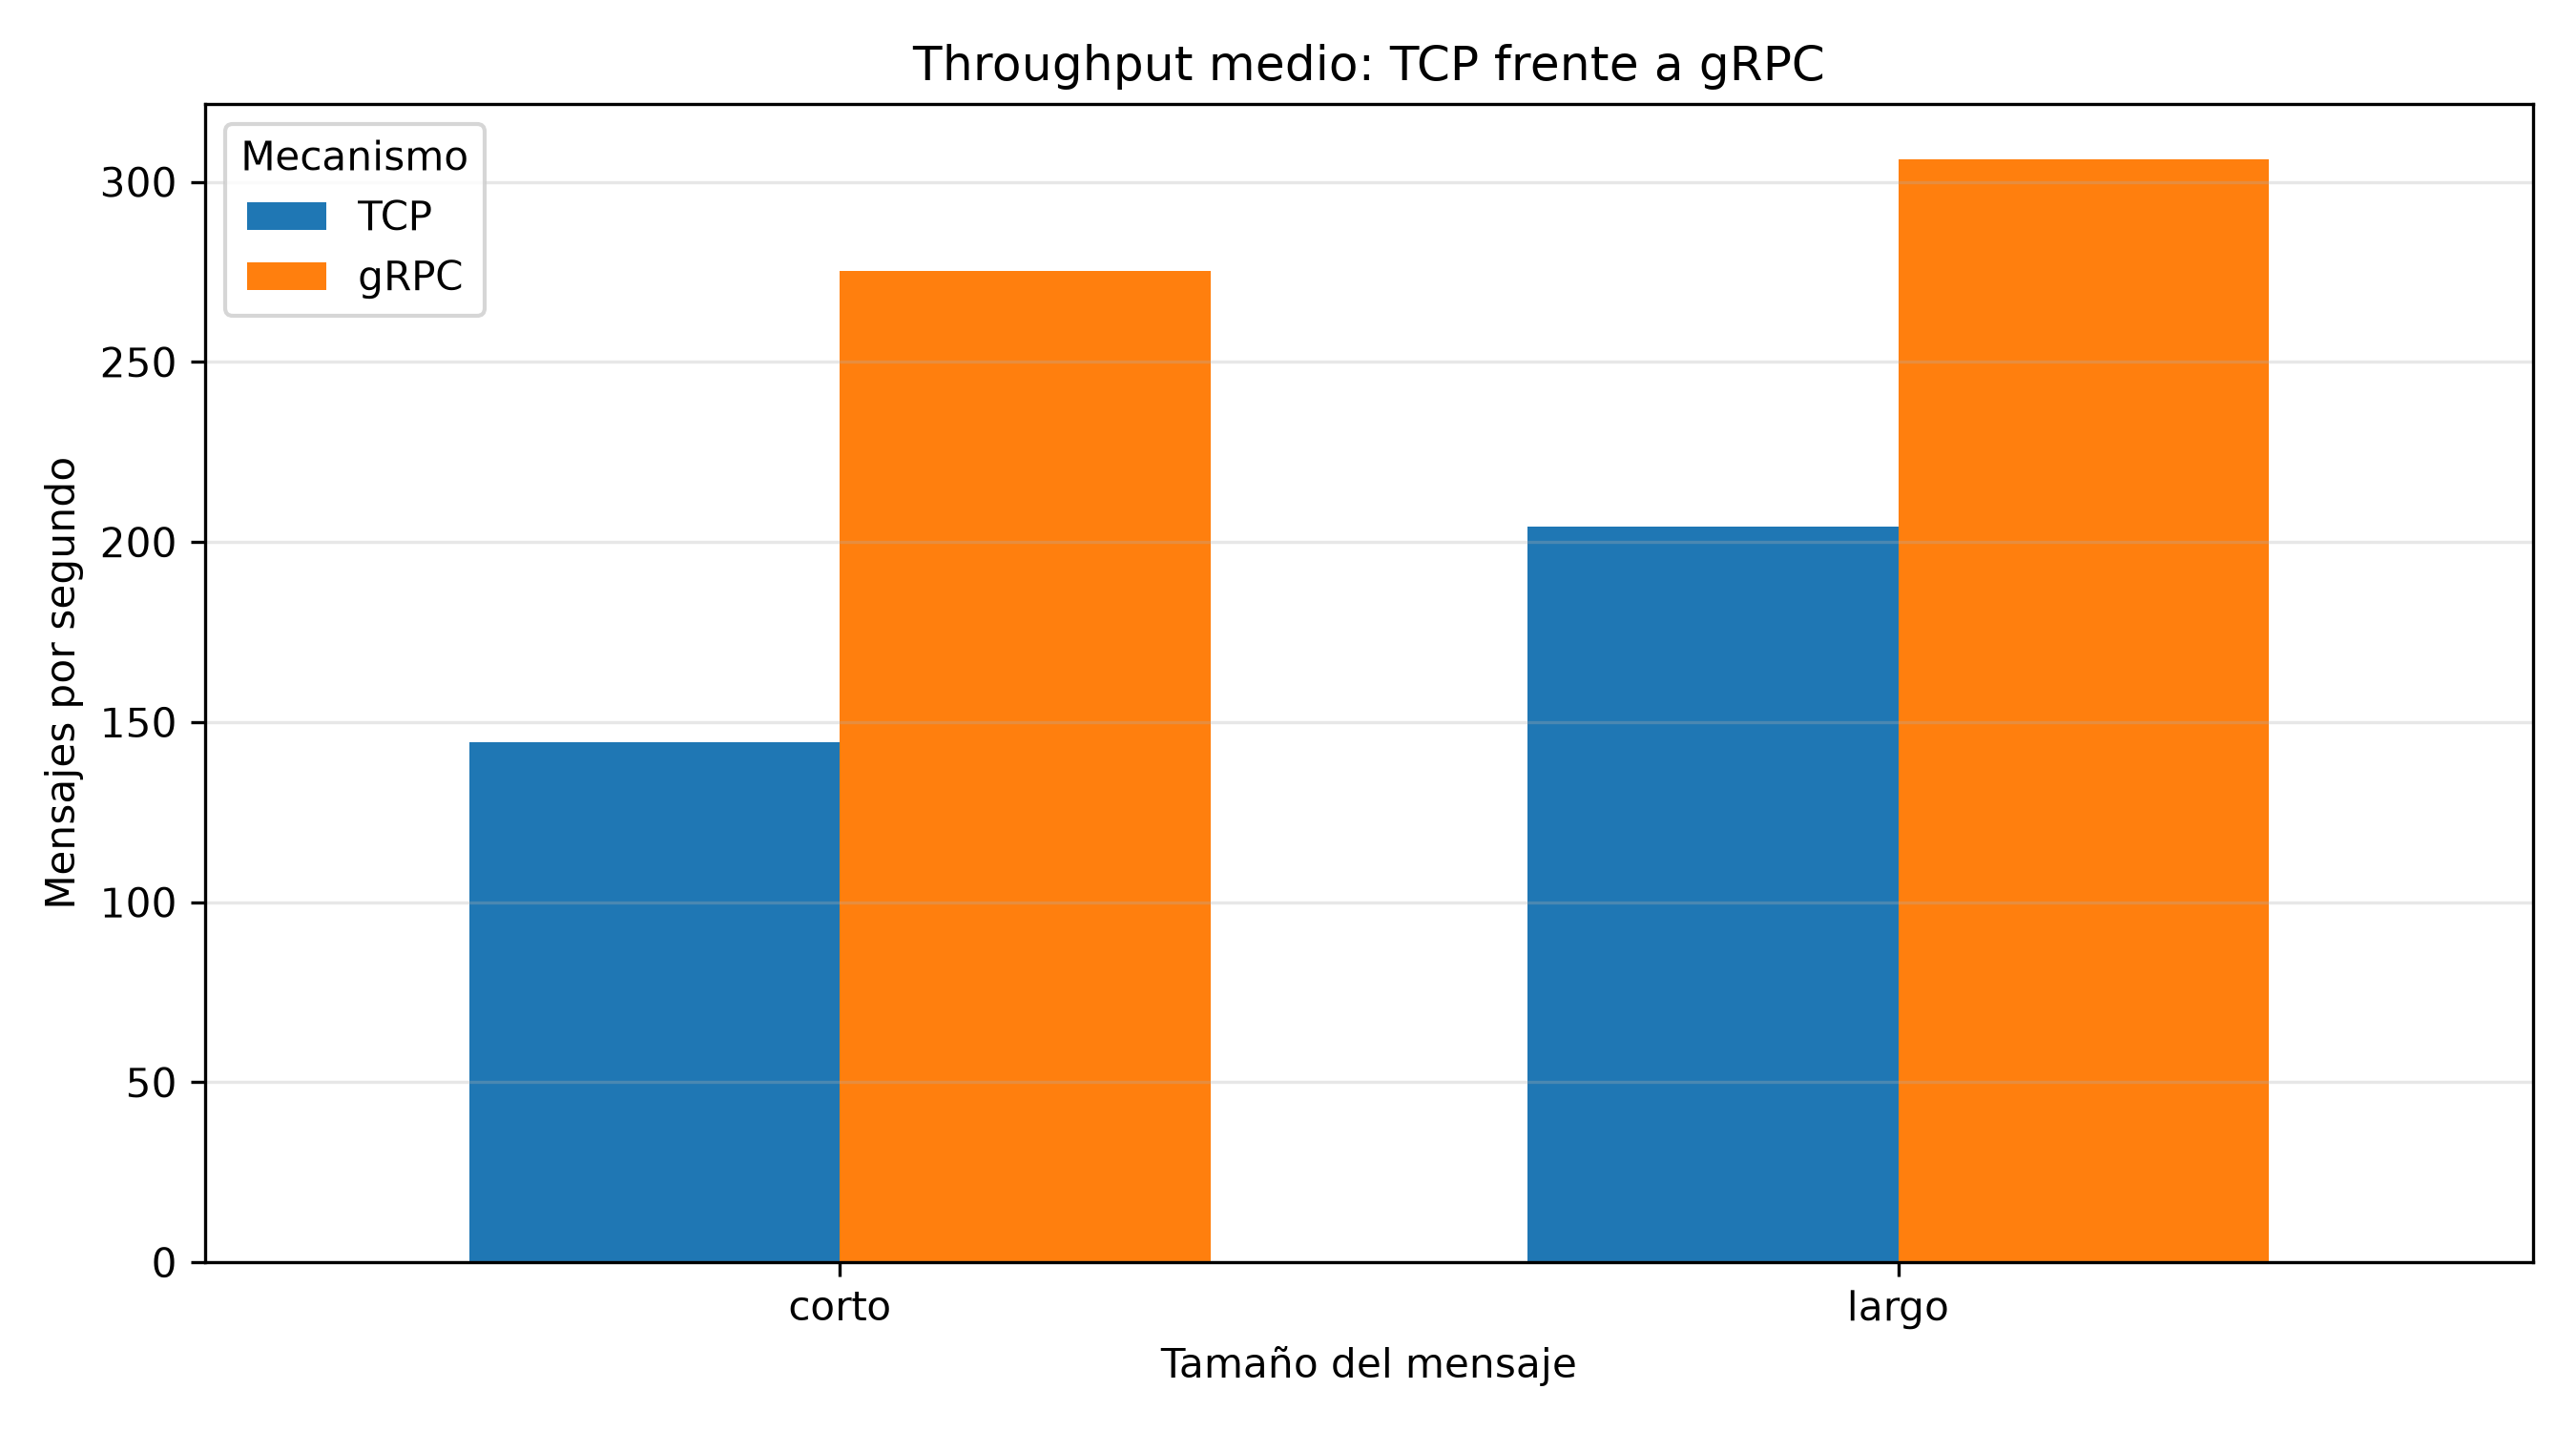
\includegraphics[width=0.85\linewidth]
{analysis/figures/comparative_throughput.png}
\caption{Comparación del throughput promedio.}
\label{fig:comparative-throughput}
\end{figure}

La Figura~\ref{fig:comparative-throughput} muestra que gRPC obtuvo
mayores valores de throughput para los dos tamaños de mensaje
evaluados, coincidiendo con los resultados de la tabla comparativa.

\subsection{Discusión y limitaciones}

Al revisar los resultados en conjunto, se observa que gRPC presentó
menor latencia media y mayor throughput en las pruebas individuales.
Por otro lado, TCP obtuvo menor latencia media en la prueba de tres
solicitudes concurrentes. Esto demuestra que no basta con utilizar
una sola métrica para determinar el comportamiento de un mecanismo
de comunicación.

También es necesario considerar las condiciones en las que se
realizaron los experimentos. Los tres nodos se ejecutaron en el mismo
equipo mediante la dirección local \texttt{127.0.0.1}, por lo que
no se evaluaron las variaciones propias de una red física entre
computadoras diferentes.

Además, las pruebas de concurrencia se limitaron a tres solicitudes
y no permiten determinar cómo responderían las implementaciones
ante una cantidad mayor de clientes.

Por estas razones, los resultados deben interpretarse como una
comparación de las dos implementaciones bajo las condiciones
específicas del proyecto. Para obtener conclusiones más amplias
sería necesario repetir las pruebas en diferentes entornos de red
y con distintos niveles de concurrencia.
